%\documentclass[handout]{beamer}
%\usepackage{pgfpages}
%\pgfpagesuselayout{4 on 1}[a4paper, landscape, border shrink=5mm]
%\pgfpageslogicalpageoptions{1}{border code=\pgfusepath{stroke}}
%\pgfpageslogicalpageoptions{2}{border code=\pgfusepath{stroke}}
%\pgfpageslogicalpageoptions{3}{border code=\pgfusepath{stroke}}
%\pgfpageslogicalpageoptions{4}{border code=\pgfusepath{stroke}}
\documentclass{beamer}
%\usetheme{nesl}  % Now it's a beamer presentation with the NESL theme!
\usetheme{Warsaw}
\usepackage{tikz}
\usetikzlibrary{shapes,arrows}
\usepackage{url}
\usepackage{movie15}
\usepackage{verbatim}
\usefonttheme{serif}

% Make a new command that will make a new subsection and a frame with the same title
\newcommand{\fst}[2]{\subsection{#1}\frame{\frametitle{#1} #2}}

% Standard LaTeX stuff - note the optional abbreviated title being provided
\title{Recent upgrades and improvements of WRF 4D-Var system}
\author[Zhang et al.]{Xin Zhang \and 
\and Ning Pan \and Qiang Cheng \and \\
Xiang-Yu Huang \and Junmei Ban}

\date{~\\
~\\
~\\\tiny{91st AMS Annual Meeting, Seattle,WA}\\
  ~\\
  ~\\
  ~\\
 \tiny{NCAR is sponsored by the National Science Foundation}
}

\institute[NCAR Earth System Laboratory]{
% \url{xinzhang@ucar.edu} \\
   NCAR Earth System Laboratory \\
%  \url{ook@ucw.cz}\\
%  Charles University, Prague
}

% We want the NSF department logo
\logo{
\includegraphics[height=.5in]{nsf1.jpg}}


\begin{document}

% The title page
\frame{\titlepage}

%%%%%%%%%%%%%%%%%%%%%%%%%
\section{Current Status of WRF 4D-Var}

\begin{comment}
\frame{
\frametitle{4D-Var versus 3D-Var\\(Adopted from ECMWF training Course 2008)}
\begin{itemize}
	\item 4D-Var is comparing observations with background model fields at the correct time \pause
	\item 4D-Var can use observations from frequently reporting stations \pause
	\item The dynamics and physics of the forecast model is in an integral part of 4D-Var, so observations are used in a meteorologically more consistent way \pause
	\item 4D-Var combines observations at different times during the 4D-Var window in a way that reduces analysis error \pause
	\item 4D-Var propagates information horizontally and vertically in a meteorologically more consistent way
\end{itemize}
}
\end{comment}

\fst{Current WRF 4D-Var}{
\begin{itemize}
	\item WRF 4D-Var was firstly released in April, 2009 with V3.1. \pause
	\item WRF adjoint and tangent linear codes (WRFPLUS) were developed based on WRF V2.0.2 around 2005. \pause
	\item Multiple Program Multiple Data (MPMD) framework, needs 3 executables: WRFDA, WRFNL and WRFPLUS. \pause
	\item Simplified physical packages: surface drag, large scale condensation and a cumulus parameterization schemes ( Q. Xiao).\pause
	\item Weak constraint with digital filter.
\end{itemize}
}

\fst{Why upgrade ?}{
\begin{itemize}
	\item Numerous bug fixes, upgrades and improvements in WRF model since 2005. V3.3 is coming\dots.\pause
	\item Particularly, WRF infrastructure changes invalid some interfaces in WRFPLUS, such as the boundary variables can not be read in anymore.\pause
	\item MPMD WRF 4D-Var is too complicate, most of the community users could not get it run without help. \pause
	\item Very high disk IO overhead associated with the number of processors.\pause
	\item Only runs good on IBM machines; unstable on other platforms and compilers.\pause
	\item 4D-Var support for Prepbufr and radiance bufr data is not clear. \pause
	\item Hard to do a complete adjoint check due to initial design of framework.
\end{itemize}
}


%%%%%%%%%%%%%%%%%%%%%%%%%%%%%%%%%
\section{Next generation WRF 4D-Var}

\fst{Upgrading WRFPLUS}{
\begin{itemize}
   	\item New WRF adjoint and tangent linear codes based on the latest WRF repository codes. \pause
	\item Constructed interfaces through which other applications can call WRF adjoint and tangent linear model directly. \pause 
	\item Testing the code on various  platforms and compilers ( IBM, Linux, Mac : xlf, g95, pgi, intel, gfortran). \pause
	\item Capability to do tangent linear and adjoint test over any length of time window. \pause 
	\item New WRFPLUS can be used as a standalone tool or as a component in 4D-Var system.
\end{itemize}
}

\begin{frame}[fragile]
\frametitle{Sample Tangent Linear and Adjoint Check of WRFPLUS }
\setbeamercolor{postit}{fg=black, bg=yellow}
\begin{beamerboxesrounded}[ lower=postit,shadow=true]{Tangent linear check:6 hours}
{\tiny
\begin{verbatim}
alpha_m=.1000E+00  coef=   0.98186174930325E+00  val_n= 0.3725210E+11  val_l= 0.3794027E+11
alpha_m=.1000E-01  coef=   0.99807498026522E+00  val_n= 0.3786723E+09  val_l= 0.3794027E+09
alpha_m=.1000E-02  coef=   0.99970559707666E+00  val_n= 0.3792910E+07  val_l= 0.3794027E+07
alpha_m=.1000E-03  coef=   0.99992019503144E+00  val_n= 0.3793724E+05  val_l= 0.3794027E+05
alpha_m=.1000E-04  coef=   0.10000447262220E+01  val_n= 0.3794196E+03  val_l= 0.3794027E+03
alpha_m=.1000E-05  coef=   0.99999981575068E+00  val_n= 0.3794026E+01  val_l= 0.3794027E+01
alpha_m=.1000E-06  coef=   0.99999998152933E+00  val_n= 0.3794027E-01  val_l= 0.3794027E-01
alpha_m=.1000E-07  coef=   0.99999990980017E+00  val_n= 0.3794026E-03  val_l= 0.3794027E-03
alpha_m=.1000E-08  coef=   0.99999956711797E+00  val_n= 0.3794025E-05  val_l= 0.3794027E-05
alpha_m=.1000E-09  coef=   0.10000030220656E+01  val_n= 0.3794038E-07  val_l= 0.3794027E-07
alpha_m=.1000E-10  coef=   0.99996176999678E+00  val_n= 0.3793882E-09  val_l= 0.3794027E-09
\end{verbatim}
}
\end{beamerboxesrounded}
\begin{beamerboxesrounded}[ lower=postit,shadow=true]{Adjoint check: 6 hours}
{\tiny
\begin{verbatim}
 ad_check: VAL_TL:    0.42476489986911E+11
 ad_check: VAL_AD:    0.42476489986912E+11
\end{verbatim}
}
\end{beamerboxesrounded}
\end{frame}

\subsection{Single executable 4D-Var}
\begin{frame}[fragile]
\frametitle{Single executable 4D-Var}
WRFPLUS includes WRF NL, AD and TL model and they are used as a subroutine in WRF 4D-Var, other than being called via shell scripts.
~\\
~\\
\setbeamercolor{postit}{fg=black, bg=yellow}
\begin{beamerboxesrounded}[ lower=postit,shadow=true]{Nonlinear call}
\begin{verbatim}
old         call da_system ("da_run_wrf_nl.ksh")
new         call da_nl_model
\end{verbatim}
\end{beamerboxesrounded}
\begin{beamerboxesrounded}[ lower=postit,shadow=true]{Tangent linear call}
\begin{verbatim}
old         call da_system ("da_run_wrfplus_tl.ksh")
new         call da_tl_model
\end{verbatim}
\end{beamerboxesrounded}
\begin{beamerboxesrounded}[ lower=postit,shadow=true]{Adjoint call}
\begin{verbatim}
old         call da_system ("da_run_wrfplus_ad.ksh")
new         call da_ad_model
\end{verbatim}
\end{beamerboxesrounded}
\end{frame}

\begin{frame}[fragile]
\frametitle{Memory exchange}
The information (TL perturbation, adjoint forcing, basic states and gradient) is exchanged via linked lists.
~\\
~\\
\setbeamercolor{postit}{fg=black, bg=yellow}
\begin{beamerboxesrounded}[ lower=postit,shadow=true]{Read basic states}
\begin{verbatim}
call domain_clock_get( grid, current_timestr=timestr )
call da_read_basicstates ( xbx, grid, ... )
\end{verbatim}
\end{beamerboxesrounded}
\begin{beamerboxesrounded}[ lower=postit,shadow=true]{Save TL perturbation}
\begin{verbatim}
call push_tl_pert (timestr)
\end{verbatim}
\end{beamerboxesrounded}
\begin{beamerboxesrounded}[ lower=postit,shadow=true]{Save AD forcing}
\begin{verbatim}
call push_ad_forcing (timestr)
\end{verbatim}
\end{beamerboxesrounded}
\end{frame}

\frame{
\frametitle{Parallel run using all processors}
4D-Var is a sequential algorithm. However, the current parallel WRF 4D-Var constructed on the Multiple Program Multiple Data mode, which have to split the total processors into 3 subsets for DA, NL and AD/TL. Lots of CPU time are wasted
\begin{center}
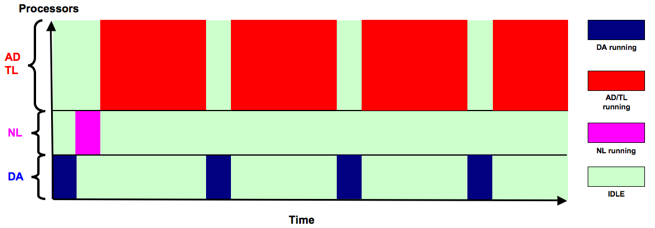
\includegraphics[scale=0.5]{mpmd_wrf4dvar}
\end{center}
}

\frame{
\frametitle{Parallel run using all processors}
Benefit from the single executable framework, every CPU is working at any time. No IDLE any more.
\begin{center}
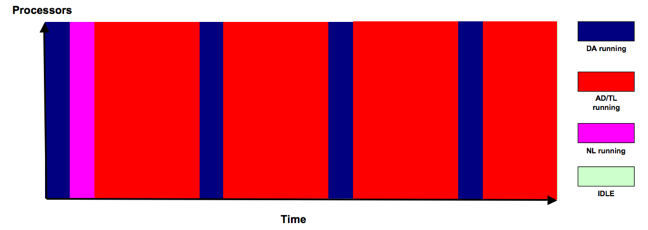
\includegraphics[scale=0.5]{single_exe_wrf4dvar}
\end{center}
}

\begin{comment}
\frame{
\frametitle{Performance improvement WRF 4DVar framework only}
\begin{itemize}
	\item $90x60x41@60km$, 6h window, 1h obs\_bin
	\item 27 iterations FGAT, NCAR bluefire (IBM P6)
\end{itemize}
\begin{center}
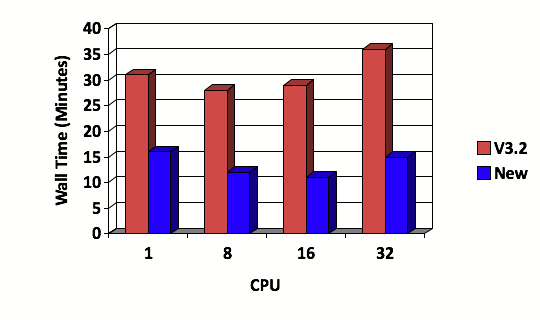
\includegraphics[scale=0.5]{small_case_performance}
\end{center}
}
\end{comment}

\frame{
\frametitle{Performance improvement WRF 4DVar framework only}
\begin{itemize}
	\item $270x180x41@20km$,6h window, 1h obs\_bin, 10 iterations
	\item 10 iterations FGAT, NCAR bluefire (IBM P6)
\end{itemize}
\begin{center}
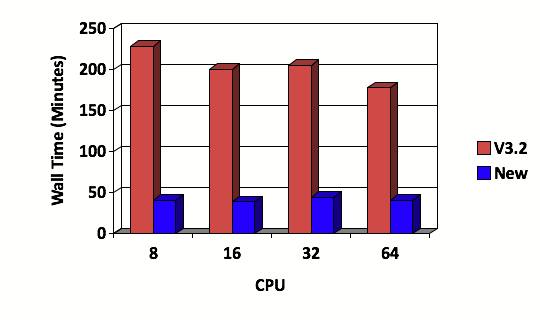
\includegraphics[scale=0.5]{big_case_performance}
\end{center}
}

\begin{comment}
\fst{Weak constraint with digital filter (enhanced)}{
\begin{tabular}{l p{2in}}
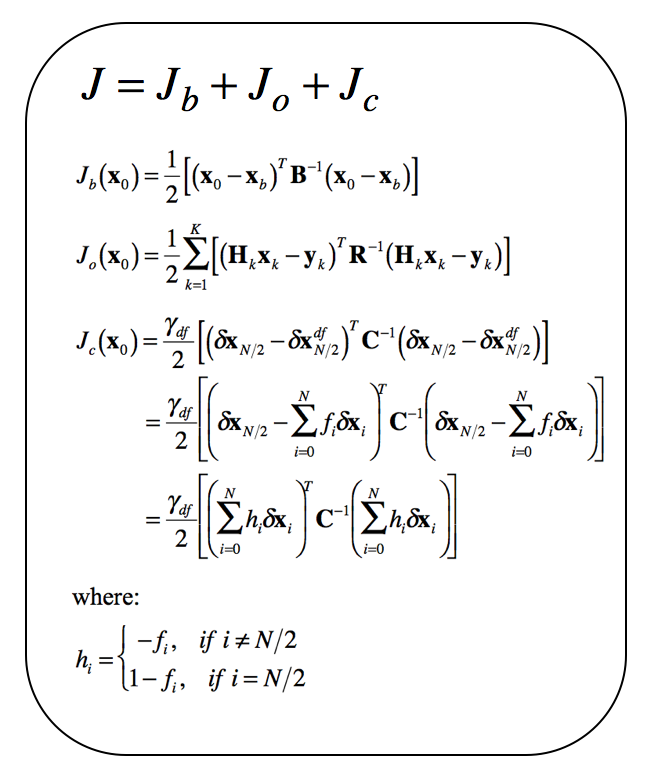
\includegraphics[scale=0.25]{jcdf_formular} \pause & 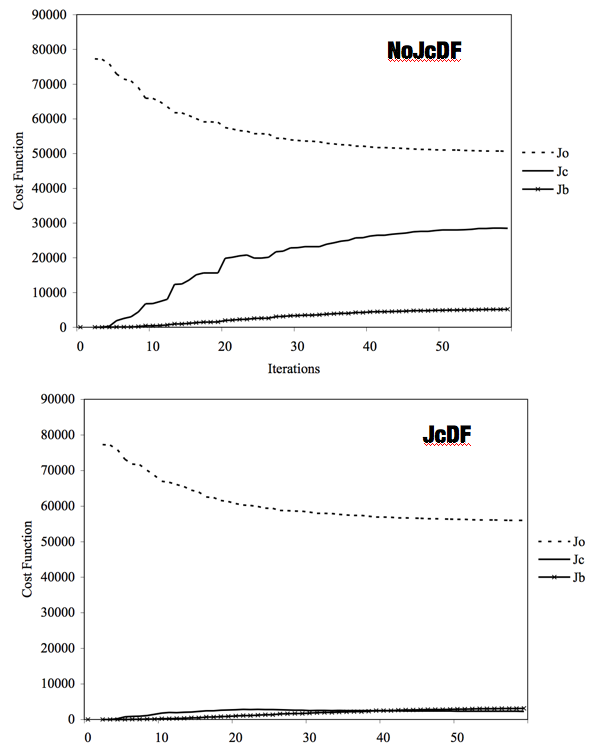
\includegraphics[scale=0.25]{jcdf}
\end{tabular}
}

\frame{
\frametitle{Weak constraint with digital filter \\(domain averaged surface pressure variation) }
\begin{center}
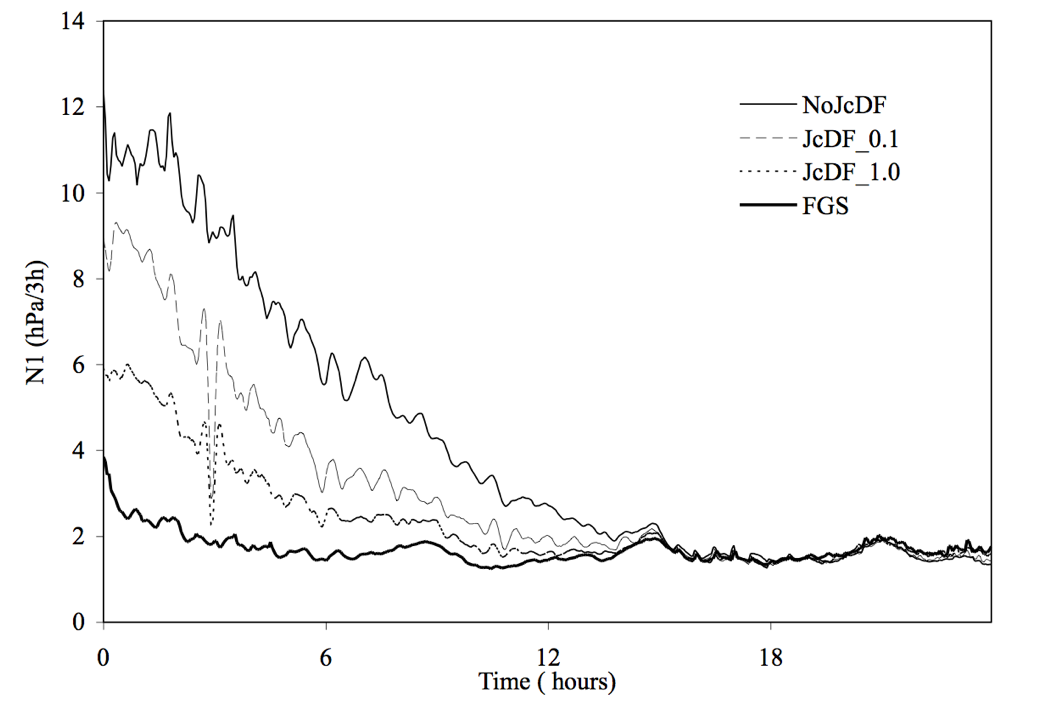
\includegraphics[scale=0.25]{jcdf_ps}
\end{center}
}
\end{comment}

\fst{Consider Lateral boundary condition as control variable}{
\begin{equation*}
J=J_b+J_o+J_c+\color{red}J_{lbc}
\end{equation*}
\begin{eqnarray*}
J_{lbc} & = & \frac{1}{2}(\mathbf{x}(t_k)-\mathbf{x}_b(t_k))^T\mathbf{B}^{-1}(\mathbf{x}(t_k)-\mathbf{x}_b(t_k))\\
& = & \frac{1}{2}\delta\mathbf{x}(t_k)^T\mathbf{B}^{-1}\delta\mathbf{x}({t_k})
\end{eqnarray*}
$J_{lbc}$ is the $J_b$ at the end of the assimilation window \\
lateral boundary control is obtained through
\begin{eqnarray*}
\frac {\partial{\delta{\mathbf{x}}_{lbc}}} {\partial{t}}=\frac{\delta\mathbf{x}(t_k)-\delta\mathbf{x}(t_0)}{t_k-t_0}
\end{eqnarray*}
}

\begin{comment}
\fst{Observations used by 4D-Var}{
\begin{itemize}
	\item Conventional observational data (little\_r, prepbufr)
	\item Radar radial velocity
	\item Radiance satellite data
\end{itemize}
\begin{center}
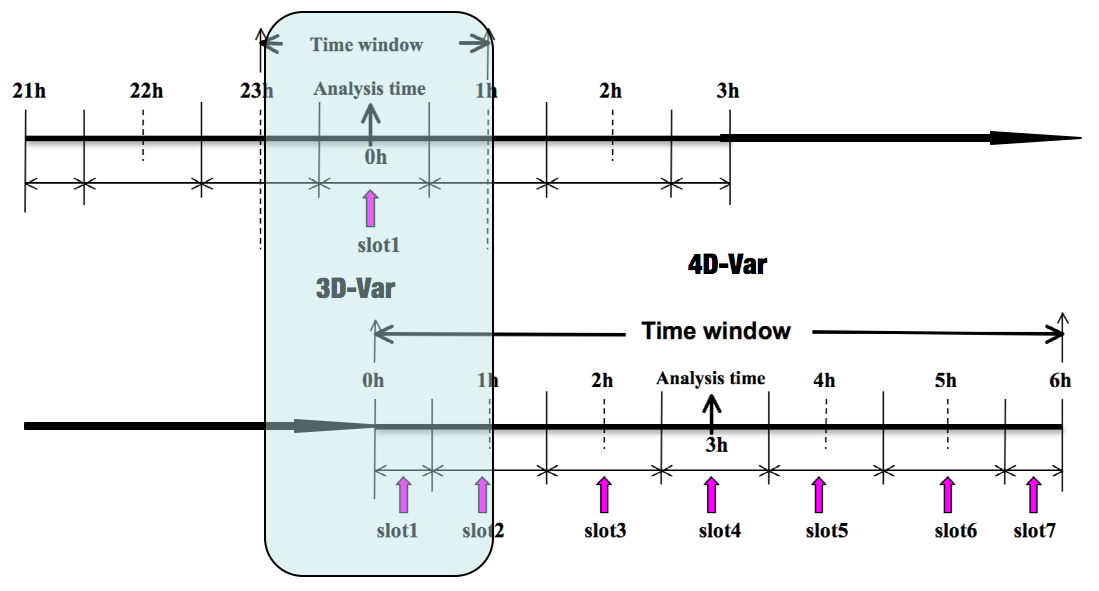
\includegraphics[scale=0.25]{obs_3dvar} \pause
\vspace {-13.61em} 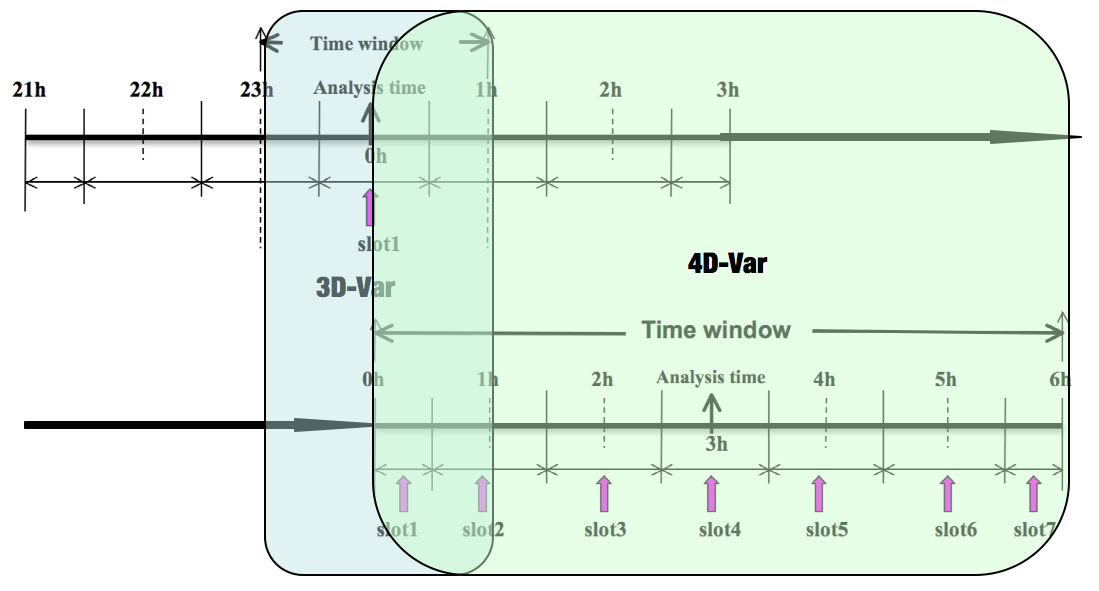
\includegraphics[scale=0.25]{obs_4dvar}
\end{center} 
}
\end{comment}

%%%%%%%%%%%%%%%%%%%%%%%%%
\section{WRF 4D-Var System Validation}

\fst{Single observation experiments}{
\begin{itemize}
	\item Initial time: $2000\_01\_25\_00:00:00$
	\item Ending time: $2000\_01\_25\_06:00:00$
	\item Observation: 500 mb Temperature at {\color{red}ending time} \\
	          $O-B=-1.168K$
	\item To investigate the difference at {\color{red}ending time} between the forecast from analysis and from background.
\end{itemize}
}

\frame{
\begin{columns}[c]
\column{5cm}
\includemovie[
  controls,poster={centerlbcjcdf.pdf},
  text={\large(Click to start the movie)\hspace*{400pt}}
]{6.0cm}{7.5cm}{centerlbcjcdf.mpeg}
\column[c]{3.5cm}
\begin{block}{Remarks}
\tiny{Forecasted 500mb T difference \\(DA forecast - reference forecast)}
\begin{itemize}
	\item {\color{red}$\star$} is the location of obs. at the ending time (6h).
	\item \tiny{JcDF is turned on}
	\item \tiny{LBC control is turned on}
	\item \tiny{Initial perturbation is on the upstream of the obs.}
	\item \tiny{Evolved perturbation at 6h hit the obs. location}
\end{itemize}
\end{block}
\end{columns}
}

\frame{
\begin{columns}[c]
\column{5cm}
\includemovie[
  controls,poster={centernolbcjcdf.pdf},
  text={\large(Click to start the movie)\hspace*{400pt}}
]{6.0cm}{7.5cm}{centernolbcjcdf.mpeg}
\column[c]{3.5cm}
\begin{block}{Remarks}
\tiny{Forecasted 500mb T difference \\(DA forecast - reference forecast)}
\begin{itemize}
	\item {\color{red}$\star$} is the location of obs. at the ending time (6h).
	\item \tiny{JcDF is turned on}
	\item \tiny{LBC control is  {\color{red}turned off}}
	\end{itemize}
\end{block}
\end{columns}
}

\frame{
\frametitle{Additional experiments design\\Observation close to boundary}
To investigate the impact of including boundary condition in data assimilation, the 6h observation is close to boundary and downstream of the boundary, we expect that the analysis response at 0h should be in boundary condition other than initial condition.
}

\frame{
\begin{columns}[c]
\column{5cm}
\includemovie[
  controls,poster={boundarylbcjcdf.pdf},
  text={\large(Click to start the movie)\hspace*{400pt}}
]{6.0cm}{7.5cm}{boundarylbcjcdf.mpeg}
\column[c]{3.5cm}
\begin{block}{Remarks}
\tiny{Forecasted 500mb T difference \\(DA forecast - reference forecast)}
\begin{itemize}
	\item {\color{red}$\star$} is the location of obs. at the ending time (6h).
	\item \tiny{JcDF is turned on}
	\item \tiny{$O-B=-0.95K$}
	\item \tiny{LBC control is {\color{red}turned on}}
	\item \tiny{Main initial perturbation is in the boundary condition other than in the initial condition ( south boundary, invisible here)}
	\item \tiny{Evolved perturbation is coming from boundary}
\end{itemize}
\end{block}
\end{columns}
}

\frame{
\begin{columns}[c]
\column{5cm}
\includemovie[
  controls,poster={boundarynolbcjcdf.pdf},
  text={\large(Click to start the movie)\hspace*{400pt}}
]{6.0cm}{7.5cm}{boundarynolbcjcdf.mpeg}
\column[c]{3.5cm}
\begin{block}{Remarks}
\tiny{Forecasted 500mb T difference \\(DA forecast - reference forecast)}
\begin{itemize}
	\item {\color{red}$\star$} is the location of obs. at the ending time (6h).
	\item \tiny{JcDF is turned on}
	\item \tiny{LBC control is {\color{red}turned off}}
	\item \tiny{Main Initial perturbation is in the location of the obs., it is fake}
	\item \tiny{Evolved perturbation at 6h is moving out from the obs. location}
\end{itemize}
\end{block}
\end{columns}
}

\begin{comment}
\frame{
\begin{columns}[c]
\column{5cm}
\includemovie[
  controls,autoresume,poster,
  text={\small(Loading boundarylbcnojcdf.mpeg)}
]{6.0cm}{7.5cm}{boundarylbcnojcdf.mpeg}
\column[c]{3.5cm}
\begin{block}{Remarks}
\tiny{Forecasted 500mb T difference \\(DA forecast - reference forecast)}
\begin{itemize}
	\item {\color{red}$\star$} is the location of obs. at the ending time (6h).
	\item \tiny{JcDF is {\color{red}turned off}}
	\item \tiny{LBC control is turned on}
	\item \tiny{Noise development dominate the domain, the perturbation development is totally different, hard to see the impact of boundary.}
\end{itemize}
\end{block}
\end{columns}
}
\end{comment}

\fst{An OSSE radar data assimilation with WRF 4D-Var \small{ (Yongrun Guo and Jenny Sun) }}{

\begin{itemize}
	\item TRUTH ----- Initial condition from TRUTH (13-h forecast initialized at 	   
                           2002061212Z from AWIPS 3-h analysis) run cutted by ndown, 	     
                           boundary condition from NCEP GFS data. \pause
	\item NODA -----  Both initial condition and boundary condition from NCEP GFS data.\pause
	\item 3DVAR -----3DVAR analysis at 2002061301Z used as the initial condition, and  
                           boundary condition from NCEP GFS. Only Radar radial velocity at  
                           2002061301Z assimilated (total data points = 97,033), 3 outer loops.\pause
	\item 4DVAR ----- 4DVAR analysis at 2002061301Z used as initial condition, and 
                           boundary condition from NCEP GFS. The radar radial velocity at 4  
                           times: 200206130100, 05, 10, and 15, are assimilated (total
                           data points = 384,304), 3 outer loops.
\end{itemize}
}


\fst{OSSE 3rd hour precipitation simulation}{
\begin{tabular}{l r}
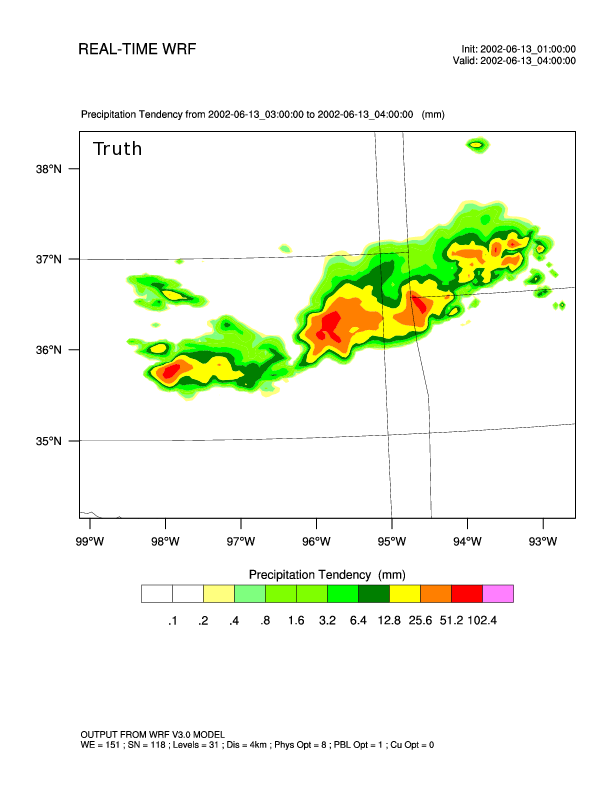
\includegraphics[scale=0.20, trim=1 240 3 100, clip]{radar_truth} & 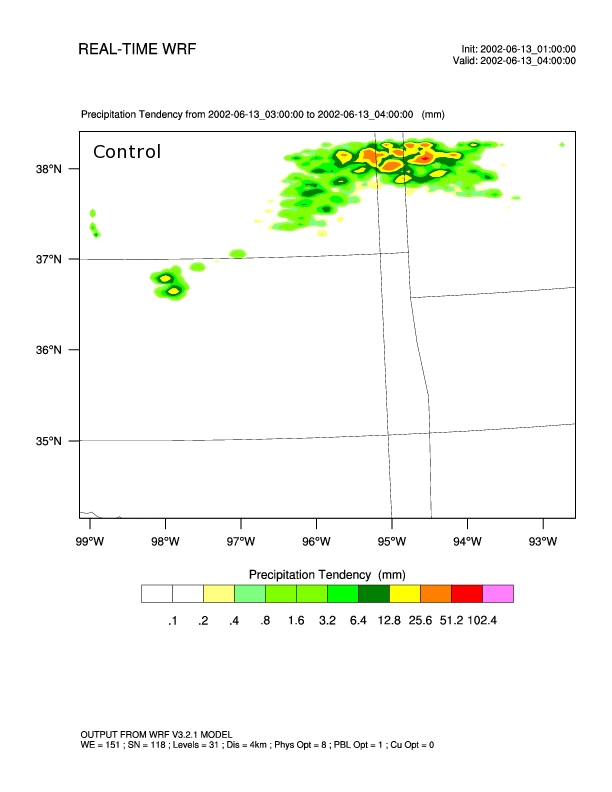
\includegraphics[scale=0.20, trim=1 240 3 100, clip]{radar_control} \\
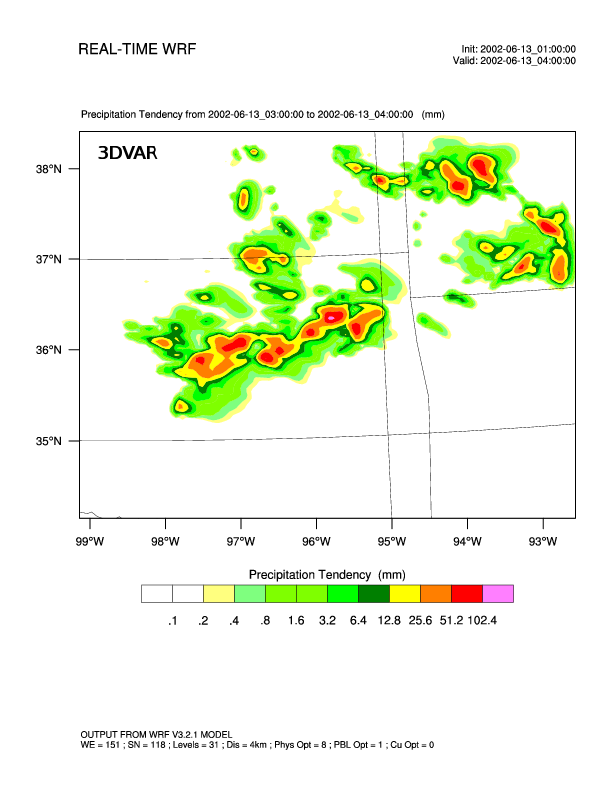
\includegraphics[scale=0.20, trim=1 160 3 130, clip]{radar_3dvar} & 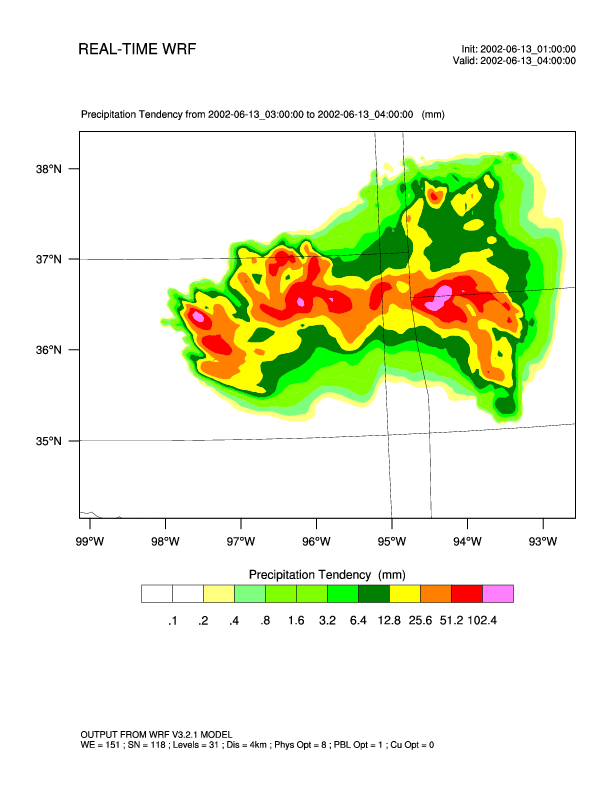
\includegraphics[scale=0.20, trim=1 160 3 130, clip]{radar_4dvar}
\end{tabular}
}

\frame{
\frametitle{Remarks}
\begin{itemize}
	\item Obviously, 4DVar reproduce the best squall line precipitation band.\pause
	\item However, the coverage and intensity of the precipitation are more than the observation.\pause
	\item Possible reason: The new WRFPLUS is a dynamic-only model, PBL and microphysics are needed.
\end{itemize}
}


%%%%%%%%%%%%%%%%%%%%%%%%%%%%%%%%%
\section{Summary}

\frame{
\frametitle{Summary}
\begin{itemize}
	\item The single executable WRF 4DVar system was developed and has showed promising performance.\\
	         Poster 541: "Evaluation of WRFDA 4D-VAR through Month-long Run and Case Study" by Xiaoyan Zhang et al. \pause 
	\item The new WRF 4DVar system has the capability to assimilate conventional observational data (little\_r or prepbufr format),radiance in bufr format and radar data. \pause
	\item The new WRF 4DVar system is able to consider lateral boundary condition as control variable and digital filter can be used as a weak constraint to suppress the high frequency noise.
\end{itemize}
}

\frame{
\frametitle{Under development}
\begin{itemize}
	\item Add simplified physics packages into WRFPLUS: surface drag, large scale condensation, a simplified moist cumulus scheme, as well as a radiation scheme.\pause
	\item Parallelization of WRF tangent linear code has been done. We are working on the parallelization of WRF adjoint codes.
\end{itemize}
}

\begin{comment}
\begin{frame}[fragile]
\frametitle{Quick Start}
Install WRFPLUS and WRFPLUS
   \begin{itemize}
        	\item WRFPLUS : WRF adjoint and tangent linear codes
		\begin{verbatim}
	         > configure [-d] wrfplus
	         > compile em_real
	         \end{verbatim}
	\item Set the the $WRFPLUS\_DIR$ environmental variable, it will be used in WRFDA compilation
		\begin{verbatim} 
		> setenv WRFPLUS_DIR full_path_of_wrfplus  
		\end{verbatim}
	\item WRFDA
		\begin{verbatim}
		> configure [-d] 4dvar
		> compile all_wrfvar
		\end{verbatim}
    \end{itemize}
\end{frame}
\end{comment}

%%%%%%%%%%%%%%%%%%%%%%%%%%%%%%%%%%%
\fst{}{
\begin{center}
~\\
~\\
~\\
~\\
~\\
{\huge{\color{red}Thank You}}\\
~\\
~\\
~\\
~\\
~\\
{\tiny{\color{blue}The NESL Mission is: \\
To advance understanding of weather, climate, atmospheric composition and processes;\\
To provide facility support to the wider community; and, \\
To apply the results to benefit society.\\}}
~\\
{\small{NCAR is sponsored by the National Science Foundation}}
\end{center}
}

\end{document}
